\documentclass[t,aspectratio=169, 8pt]{beamer}
\usetheme{baurg}
\usepackage{rg-code-beamer}

\usepackage[english]{babel}
\usepackage{subcaption}
% Maths and Physics
\usepackage{amsmath}
\usepackage{amsthm}
\usepackage{amssymb}
\usepackage{physics}
\usepackage{tabularx}
\usepackage{braket}
\usepackage{bm}
\usepackage{array,multirow,graphicx}


\def\*#1{\bm{#1}}

% For figures
\usepackage{tikz}
\usetikzlibrary{decorations.pathmorphing}
\usetikzlibrary{shapes}
\usetikzlibrary{matrix,shapes.geometric}
\usetikzlibrary{positioning,fit,calc} 
\usepackage{svg}
\usepackage{subcaption}

\title{Brute Force Awakens}
\subtitle{April 9, 2021}
\author{Ruben Gerritsen}
\department{CASA Day - Episode V}


\begin{document}

\begin{titleframe}[variant=1,bgimage=background.png]
\end{titleframe}

% 1 %
\begin{frame}[fragile]
	\frametitle{Overview}
	\begin{itemize}
		\item What is it about?
		\item Multiscale Approach
		\item Modelling Carrier Dynamics
		\item Electronic Structure Calculations
		\item How long does it take?
		\item dsd
	\end{itemize}
\end{frame}

%%%%%%%%%%%%%%%%%%%%%%%%%%%%%%%%%%%%%%%%%%%%%%%%%%%%%%%%%%%%%%%%%%%%%%%%%%%%%%%
% A PRIMER IN ORGANIC ELECTRONICS
%%%%%%%%%%%%%%%%%%%%%%%%%%%%%%%%%%%%%%%%%%%%%%%%%%%%%%%%%%%%%%%%%%%%%%%%%%%%%%%%
\begin{frame}
	\frametitle{Organic Materials and the Processes Involved}
	\begin{columns}[c]
		\begin{column}{0.6\textwidth}
			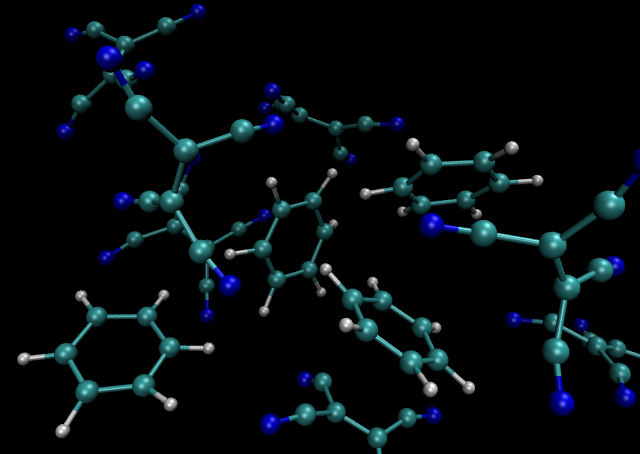
\includegraphics[height=0.7\textheight]{material.png}
		\end{column}
		\begin{column}{0.36\textwidth}
			\textbf{Particles}
			\begin{itemize}
				\item Electrons
				\item Holes
				\item Excitons
			\end{itemize}
			\medskip
			\textbf{Processes}
			\begin{itemize}
				\item Charge transfer
				\item Recombination of electrons and holes
				\item Exciton generation
				\item Exciton dissociation: via Charge Transfer (CT) states
				\item Exciton decay
				\item Exciton transfer fds
			\end{itemize}
		\end{column}
	\end{columns}
\end{frame}



%%%%%%%%%%%%%%%%%%%%%%%%%%%%%%%%%%%%%%%%%%%%%%%%%%%%%%%%%%%%%%%%%%%%%%%%%%%%%%%%
% DYNAMICS
%%%%%%%%%%%%%%%%%%%%%%%%%%%%%%%%%%%%%%%%%%%%%%%%%%%%%%%%%%%%%%%%%%%%%%%%%%%%%%%%
\title{Modelling Carrier Dynamics}
\begin{chapterframe}
	\frametitle{Modelling Carrier Dynamics}
	\begin{itemize}
		\item From Hopping Rates to a Graph
		\item The Master Equation (ME)
		\item Kinetic Monte Carlo (KMC)
	\end{itemize}
\end{chapterframe}

\begin{frame}[fragile]
	\frametitle{Code Example}
	Here is some text with a bit of code \mintinline{python}{fiets}
	\begin{minted}{python}
def initializeVelocity(sd,nrOfAtoms):
    """ Returns randomized initial velocities for the atoms, with standar
        deviation = 'sd'. """
    return(np.random.normal(0.0,sd,(nrOfAtoms,3)))
	\end{minted}
\end{frame}

%%%%%%%%%%%%%%%%%%%%%%%%%%%%%%%%%%%%%%%%%%%%%%%%%%%%%%%%%%%%%%%%%%%%%%%%%%%%%%%%
% Electronic Structure Calculations
%%%%%%%%%%%%%%%%%%%%%%%%%%%%%%%%%%%%%%%%%%%%%%%%%%%%%%%%%%%%%%%%%%%%%%%%%%%%%%%%
\title{Electronic Structure Calculations}
\begin{chapterframe}
	\frametitle{Electronic Structure Calculations}
	How do we get the parameters and values for the KMC?\\
	Answer: Quantum Mechanics\\
	\medskip
	What we will discuss next
	\begin{itemize}
		\item Describing molecules and the Born-Oppenheimer approximation
		\item Density Functional Theory (DFT)
		\item \textit{GW} method and the Bethe Salpeter Equation (BSE)
	\end{itemize}
\end{chapterframe}

\begin{frame}
	\frametitle{The Born-Oppenheimer Approximation}
	\small
	The full Schr\"odinger equation (which contains everything one would ever want to know)
	$$  \hat{H}_\text{sys} \Psi= E\Psi  \quad\quad \text{or} \quad\quad \hat{H}_\text{sys} \Psi(\{\mathbf{r}_i, \sigma_i\},\ \{Z_l,\*R_l\}) = E\Psi(\{\mathbf{r}_i, \sigma_i\},\ \{Z_l,\*R_l\})$$
	\begin{columns}[c]
		\begin{column}{0.45\textwidth}
			\footnotesize
			\begin{equation*} \label{FullHamiltonian}
				\begin{split}
					\hat{H}_\text{sys} =& \frac{1}{2}\sum_l \frac{1}{M_l}\*P_l^2 +  \frac{1}{2}\sum_i \*p_i^2 + \frac{1}{2}\sum_{\substack{l,l' \\(l \neq l')}} Z_lZ_{l'} v(\*R_l - \*R_{l'})\\
					&-\sum_l\sum_i Z_l v(\*r_i-\*R_l) + \frac{1}{2}\sum_{\substack{i,i' \\(i \neq i')}} v(\*r_i - \*r_{i'})
				\end{split}
			\end{equation*}
		\end{column}
		\begin{column}{0.5\textwidth}
			\begin{itemize}
				\item[] For benzene: 12 nuclei and 42 electrons
				\item[] = 162 spatial dimensions
				\item[] Leads to a very large system of coupled differential equations!
			\end{itemize}
		\end{column}
	\end{columns}
	The Born-Oppenheimer approximation leads to the electronic Schr\"odinger equation
	$$	\hat{H}_{e} \Psi_e(\{\mathbf{r}_i\}; \{Z_l,\*R_l\}) = E \Psi_e(\{\mathbf{r}_i\}; \{Z_l,\*R_l\})$$
	Still difficult to solve
	\begin{itemize}
		\item Still high dimensional: $3N$ spatial dimensions
		\item $\Psi$ should be normalized: $\int \abs{\Psi(\*r_1,\ldots,\*r_N)}^2 \dd{\*r^N} = 1$
		\item $\Psi$ should be anti-symmetric: $\Psi(\*r_1,\ldots,\*r_k, \*r_l ,\ldots,\*r_N) = - \Psi(\*r_1,\ldots,\*r_l ,\*r_k ,\ldots,\*r_N)$
	\end{itemize}
\end{frame}


%%%%%%%%%%%%%%%%%%%%%%%%%%%%%%%%%%%%%%%%%%%%%%%%%%%%%%%%%%%%%%%%%%%%%%%%%%%%%%%%
% QUESTIONS
%%%%%%%%%%%%%%%%%%%%%%%%%%%%%%%%%%%%%%%%%%%%%%%%%%%%%%%%%%%%%%%%%%%%%%%%%%%%%%%%
\title{Questions}
\begin{chapterframe}
	\frametitle{Questions}
	\vspace{0.5cm}
	\begin{center}
		{\fontsize{60}{64} \selectfont \bfseries{?}}
	\end{center}
\end{chapterframe}


\end{document}